\documentclass[12pt, titlepage]{article}

\usepackage{booktabs}
\usepackage{enumerate}
\usepackage{graphicx}
\usepackage{mdwlist}
\usepackage{tabularx}
\usepackage{float}
\usepackage{hyperref}
\hypersetup{
    colorlinks,
    citecolor=black,
    filecolor=black,
    linkcolor=red,
    urlcolor=blue
}
\usepackage[round]{natbib}

\title{SE 3XA3: Software Requirements Specification\\super-refactored-mario-python}

\author{Team 203, Abstract Connoiseurs
		\\ Alexander Samaha, samahaa
		\\ Daniel Noorduyn, noorduyd
		\\ David Jandric, jandricd
}

\date{\today}

%\input{../Comments}%

\begin{document}

\maketitle

\pagenumbering{roman}
\tableofcontents
\listoftables
\listoffigures

\begin{table}[bp]
\caption{\bf Revision History}
\begin{tabularx}{\textwidth}{p{3cm}p{2cm}X}
\toprule {\bf Date} & {\bf Version} & {\bf Notes}\\
\midrule
Feb 4 2020 & 1.0 & Initial changes to the document \\
Date 2 & 1.1 & Notes\\
\bottomrule
\end{tabularx}
\end{table}

\newpage

\pagenumbering{arabic}

This document describes the requirements for super-refactored-mario-python, which is an implementation of the Super Mario Bros. game in Python. The template for the Software
Requirements Specification (SRS) is a subset of the Volere
template~\citep{RobertsonAndRobertson2012}. This document serves to inform users and stakeholders of the overview of the project including constraints and objectives this project hopes to meet.

\section{Project Drivers}

\subsection{The Purpose of the Project}
    The purpose of super-refactored-mario-python is to re implement and modify the age old Super Mario Bros. game in an open source environment. The team will finish the work started and left uncompleted, then look to add features that diverge from the original game. The end result is a version of Super Mario Bros. that can be enjoyed by anyone with access to a computer with the proper libraries installed.

\subsection{The Stakeholders}

\subsubsection{The Client}
    The client for super-refactored-mario-python is the instructor and teaching assistants of the SFWRENG 3XA3 course.
\subsubsection{The Customers}
    The customers of this project are all with an interest in the original Super Mario Bros. game and open-source game development in general. This project will be available for anyone to download if they have access to a computer that satisfies the hardware and software requirements.
\subsubsection{Other Stakeholders}
    The original project owner has a vested interest in the completion of their unfinished project. This may include the integration of the changes and features put forward during the development cycle. Furthermore, the open-source Pygame community will have a vested interest in the propagation of its use to make video games. Finally, the development team also has a vested interest in the success of the project.
\subsection{Mandated Constraints}
    \textbf{Description:} The project shall use the Pygame library for Python game development.\\
    \textbf{Rationale:} The project is originally written with the Pygame library and will make it easier to continue using it.\\
    \textbf{Fit Criterion:} Running the game files with Python includes and runs the Pygame library.\\\\
    \textbf{Description:} The project shall follow the structure of deliverables outlined in the project schedule.\\
    \textbf{Rationale:} The project needs to follow a logical schedule to ensure completion of the product within the allotted time.\\
    \textbf{Fit Criterion:} The project is completed and all deliverables submitted by April 6th 2020.
    \textbf{Description:} The project shall use the Pygame library for Python game development.\\
    \textbf{Rationale:} The project is originally written with the Pygame library and will make it easier to continue using it.\\
    \textbf{Fit Criterion:} Running the game files with Python includes and runs the Pygame library.\\\\
\subsection{Naming Conventions and Terminology}
    \textbf{SFWRENG 3XA3} - The Software Engineering Practice and Experience: Software Project Management course instructed by Dr. Asghar Bokhari.\\
    \textbf{Super Mario Bros.} - The original arcade game released in 1985 for the Nintendo Entertainment System in North America.\\
    \textbf{Pygame} - Popular library for small open-source games written in Python.\\
    \textbf{Koopa} - Refers to a non-playable character in the Super Mario Bros. game that is encountered as an enemy. This character has a shell that can be used as a projectile.\\
    \textbf{Regular enemy} - Refers to a non-playable character in the Super Mario Bros. game that is encountered as an enemy such as a Goomba.\\
\subsection{Relevant Facts and Assumptions}
    \subsubsection{Facts}
    \begin{itemize}
        \item Pygame is a set of modules used to create video games written in Python. It encompasses graphics and sound libraries.
        \item The original repository contains 1390 lines of Python code.
    \end{itemize}
    \subsubsection{Assumptions}
    It is assumed that the user has access to a modern computer with the necessary Python interpreter installed along with the Pygame library and is able to run the files. Along with this, the user is expected to have working knowledge of running Python code from the command line. The user is assumed to have a keyboard and a mouse to be able to interact with the game. It is assumed that the user has installed all the required artefacts in a compatible operating system environment.
User characteristics should go under assumptions.

\section{Functional Requirements}

\subsection{The Scope of the Work and the Product}

\subsubsection{The Context of the Work}

\subsubsection{Work Partitioning}

\subsubsection{Individual Product Use Cases}
The primary use case of this product is to be played from start to end, and get the best high-score. There will be a number of levels, and each will have a high score associated with it, for players to challenge themselves and constantly improve their score.

\subsection{Functional Requirements}
\begin{enumerate}[{FR}1. ]
    \item When the user presses the 'W' key, the character shall jump.
    \item When the user presses the 'A' key, the character shall move left.
    \item When the user presses the 'S' key, the character shall duck, making the characters size half of what it is.
    \item When the user presses the 'D' key, the character shall move left.
    \item When the character is ducking, they shall be prevented from moving, until they stop ducking.
    \item When the user jumps on top of a regular enemy, they shall die.
    \item When the user jumps on a 'Koopa', the 'Koopa' shall retract into its shell.
    \item If the user walks into, or jumps onto, the 'Koopa shell', it shall start sliding across the ground, and will bounce off walls and move in the opposite direction.
    \item If the player character or enemy is hit by the shell, they shall die.
    \item If the player dies, they shall be reset to the beginning of the level and a life will be deducted.
    \item The player shall have 3 lives.
    \item If the player loses all 3 lives, they shall be returned to the main menu, and their high-score will be saved.
    \item When the player reaches a 'flagpole', they shall win the level, and be transported to the next.
    \item When the player finishes all levels in sequence, they shall be shown a 'You Win' screen, and be transported to the main menu. Their high-score shall be saved.
\end{enumerate}
\section{Non-functional Requirements}

\subsection{Look and Feel Requirements}
\begin{enumerate}[{LF}1. ]
    \item The product shall look extremely similar to the original Super Mario Bros.\\
    \textbf{Fit Criteria:} Users who identify as familiar with the original game should be able to navigate through the first level
    \item The product shall have a modern looking menu.\\
    \textbf{Fit Criteria:} Use
\end{enumerate}



\subsection{Usability and Humanity Requirements}

\subsubsection{Ease of Use Requirements}
\begin{enumerate}[{UH}1. ]
    \item The product shall be usable for anybody over the age of 10.
    \item The product shall have simple, standard controls.
\suspend{enumerate}

\subsubsection{Personalization and Internationalization Requirements}
N/A

\subsubsection{Learning Requirements}
\resume{enumerate}[{[{UH}1.]}]
    \item The product shall be playable by a user after reading the in game tutorial.
    \item The product shall be playable by some users without reading the in game tutorial.
\suspend{enumerate}

\subsubsection{Understandability and Politeness Requirements}
\resume{enumerate}[{[{UH}1.]}]
    \item The product shall use simple language which can be understandable by 95\% of users.
    \item The product shall use standard icons indicative of their function to avoid confusion of the user.
    \item The product shall use a simple font which is easily read by all users.
\end{enumerate}

\subsubsection{Accessibility Requirements}
N/A



\subsection{Performance Requirements}

\subsubsection{Speed and Latency Requirements}
\begin{enumerate}[{PR}1. ]
    \item The product shall run at 60 frames per second.
    \item The product shall take no more than 3 seconds to load and display all resources.
    \item The product shall not significantly slow down if there are 100 entities displaying on the screen.
\suspend{enumerate}

\subsubsection{Safety-Critical Requirements}
N/A

\subsubsection{Precision or Accuracy Requirements}
\resume{enumerate}[{[{PR}1. ]}]
    \item The product shall respond correctly to inputs 100\% of the time.
    \item The product shall correctly calculate the high-score 100\% of the time.
\suspend{enumerate}

\subsubsection{Reliability and Availability Requirements}
\resume{enumerate}[{[{PR}1. ]}]
    \item The product shall be able to be run by a user for at least 1 hour.
\suspend{enumerate}

\subsubsection{Robustness or Fault-Tolerance Requirements}
\resume{enumerate}[{[{PR}1. ]}]
    \item The product shall not crash if given many inputs at a time.
    \item The product shall not crash if there are under 1000 entities visible.
\suspend{enumerate}

\subsubsection{Capacity Requirements}
\resume{enumerate}[{[{PR}1. ]}]
    \item The product shall be able to handle a single user.
\suspend{enumerate}

\subsubsection{Scalability or Extensibility Requirements}
\resume{enumerate}[{[{PR}1. ]}]
    \item The product shall be easily modifiable for the addition of features.
    \item The product shall contain an easy way to add levels.
    \item The product shall be easily modifiable for the addition of enemies and blocks.
\suspend{enumerate}

\subsubsection{Longevity Requirements}
\resume{enumerate}[{[{PR}1. ]}]
    \item The product shall run until a major Python or Pygame update.
\end{enumerate}



\subsection{Operational and Environmental Requirements}

\subsubsection{Expected Physical Environment}
\begin{enumerate}[{OE}1. ]
    \item The product shall run on a personal computer.
\suspend{enumerate}

\subsubsection{Requirements for Interfacing with Adjacent Systems}
\resume{enumerate}[{[{OE}1. ]}]
    \item The product shall run on computer using Windows 10, MacOS Catalina, and Ubuntu 18.
    \item The product shall run on a computer with Python 3.7 and Pygame.
\suspend{enumerate}

\subsubsection{Productization Requirements}
\resume{enumerate}[{[{OE}1. ]}]
    \item The product shall be available on GitLab for download.
\suspend{enumerate}

\subsubsection{Release Requirements}
\resume{enumerate}[{[{OE}1. ]}]
    \item The product will have a final release in early April, 2020.
\end{enumerate}



\subsection{Maintainability and Support Requirements}

\subsubsection{Maintenance Requirements}
\begin{enumerate}[{MS}1. ]
    \item The product shall be maintained by the developers until early April, 2020.
    \item The product shall receive updates to fix bugs.
    \item The product shall be open source, and may receive updates from other programmers.
\suspend{enumerate}

\subsubsection{Supportability Requirements}
\resume{enumerate}[{[{MS}1. ]}]
    \item The product shall be supported on OS's mentioned previous.
\end{enumerate}

\subsubsection{Adaptability Requirements}
N/A



\subsection{Security Requirements}

\subsubsection{Access Requirements}
\begin{enumerate}[{SR}1. ]
    \item The products source code shall be available for any user.
\suspend{enumerate}

\subsubsection{Integrity Requirements}
\resume{enumerate}[{[{SR}1. ]}]
    \item All data shall be stored locally on the users machine.
\suspend{enumerate}

\subsubsection{Privacy Requirements}
\resume{enumerate}[{[{SR}1. ]}]
    \item The product shall not save any personal user data.
\suspend{enumerate}

\subsubsection{Audit Requirements}
N/A

\subsubsection{Immunity Requirements}
\resume{enumerate}[{[{SR}1. ]}]
    \item The developers of the project shall not provide malicious links.
    \item Official versions of the product shall only come from the developers GitLab repository.
\end{enumerate}



\subsection{Cultural Requirements}

\subsubsection{Cultural Requirements}
\begin{enumerate}[{CR}1. ]
    \item The product shall not contain any controversial content.
    \item The product shall use Canadian English spelling.
\end{enumerate}

\subsubsection{Political Requirements}
N/A



\subsection{Legal Requirements}

\subsubsection{Compliance Requirements}
\begin{enumerate}[{LR}1. ]
    \item The product shall not violate copyright.
    \item The product shall give credits to creators of any original content used by the product, that was not created by the developers.
\end{enumerate}

\subsubsection{Standards Requirements}
N/A



\subsection{Health and Safety Requirements}
\begin{enumerate}[{HS}1. ]
    \item The product shall not endanger its users in any way.
\end{enumerate}

\section{Project Issues}

\subsection{Open Issues}
A specific version of the Apple Mac-Book operation system combined with a specific version of the python language doesn't allow the Pygame library to be executed correctly. Investigation into solutions is currently being performed.

\subsection{Off-the-Shelf Solutions}
Considering this project is attempting to remake Super Mario Bros (howbeit in a unique way) there are many open source, free versions that have created to attempt something similar. These versions can be referenced to create key aspects of the game that would be shared across any re-creation attempts.

There are also the official version of Super Mario Bros that will be referenced for the creation of characters and certain desirable aspects that this project aims to mimic. However, it is key to note that there will be no code so the official game is more like a creativity mine.

Lastly, there are multiple online resources such as YouTube tutorials or coding forums that can help familiarize the development team with new tools.

The game engine called Pygame will be used to do most of the heavy processing.

\subsection{New Problems}
\subsubsection{Effects on the Current Environment}
The team cannot think of this project as a replacement for the official Super Mario Bros game, or as an improvement; it is simply a mimic with some fun twists made out of appreciation for the original.

\subsubsection{Limitations in the Implementation Environment}
Due to the fact that the development team has no experience designing and coding a game utilizing the Pygame library, issues could arise when trying to implement the game. If too many core aspects prove impossible to create it may result in the team having to choose a new library or even coding language to implement the game. This means the team must first attempt to code the base functionality of the game to determine possibility, before adding the fun aspects of the game.

\subsubsection{Problems Resulting from the Solution}
The resultant project will obviously draw heavily from the official Nintendo game. This may cause any distribution of the project to be a violation of the Digital Millennium Copyright Act.

\subsubsection{Possible User Related Issues}
A lack of accessible controls for end users with movement restrictions could pose a large issue. This would mean the team must develop alternative control methods with better accessibility. The team must factor this into the decision to publicly distribute the game.

\subsection{Tasks}
\subsubsection{Project Schedule}
A link to our project schedule can be found in the project repository linked below:
\href{https://gitlab.cas.mcmaster.ca/jandricd/super-refactored-mario-bros/tree/master/ProjectSchedule}{Link to Gantt chart and Resource chart}

\begin{figure}[H]
    \centering
    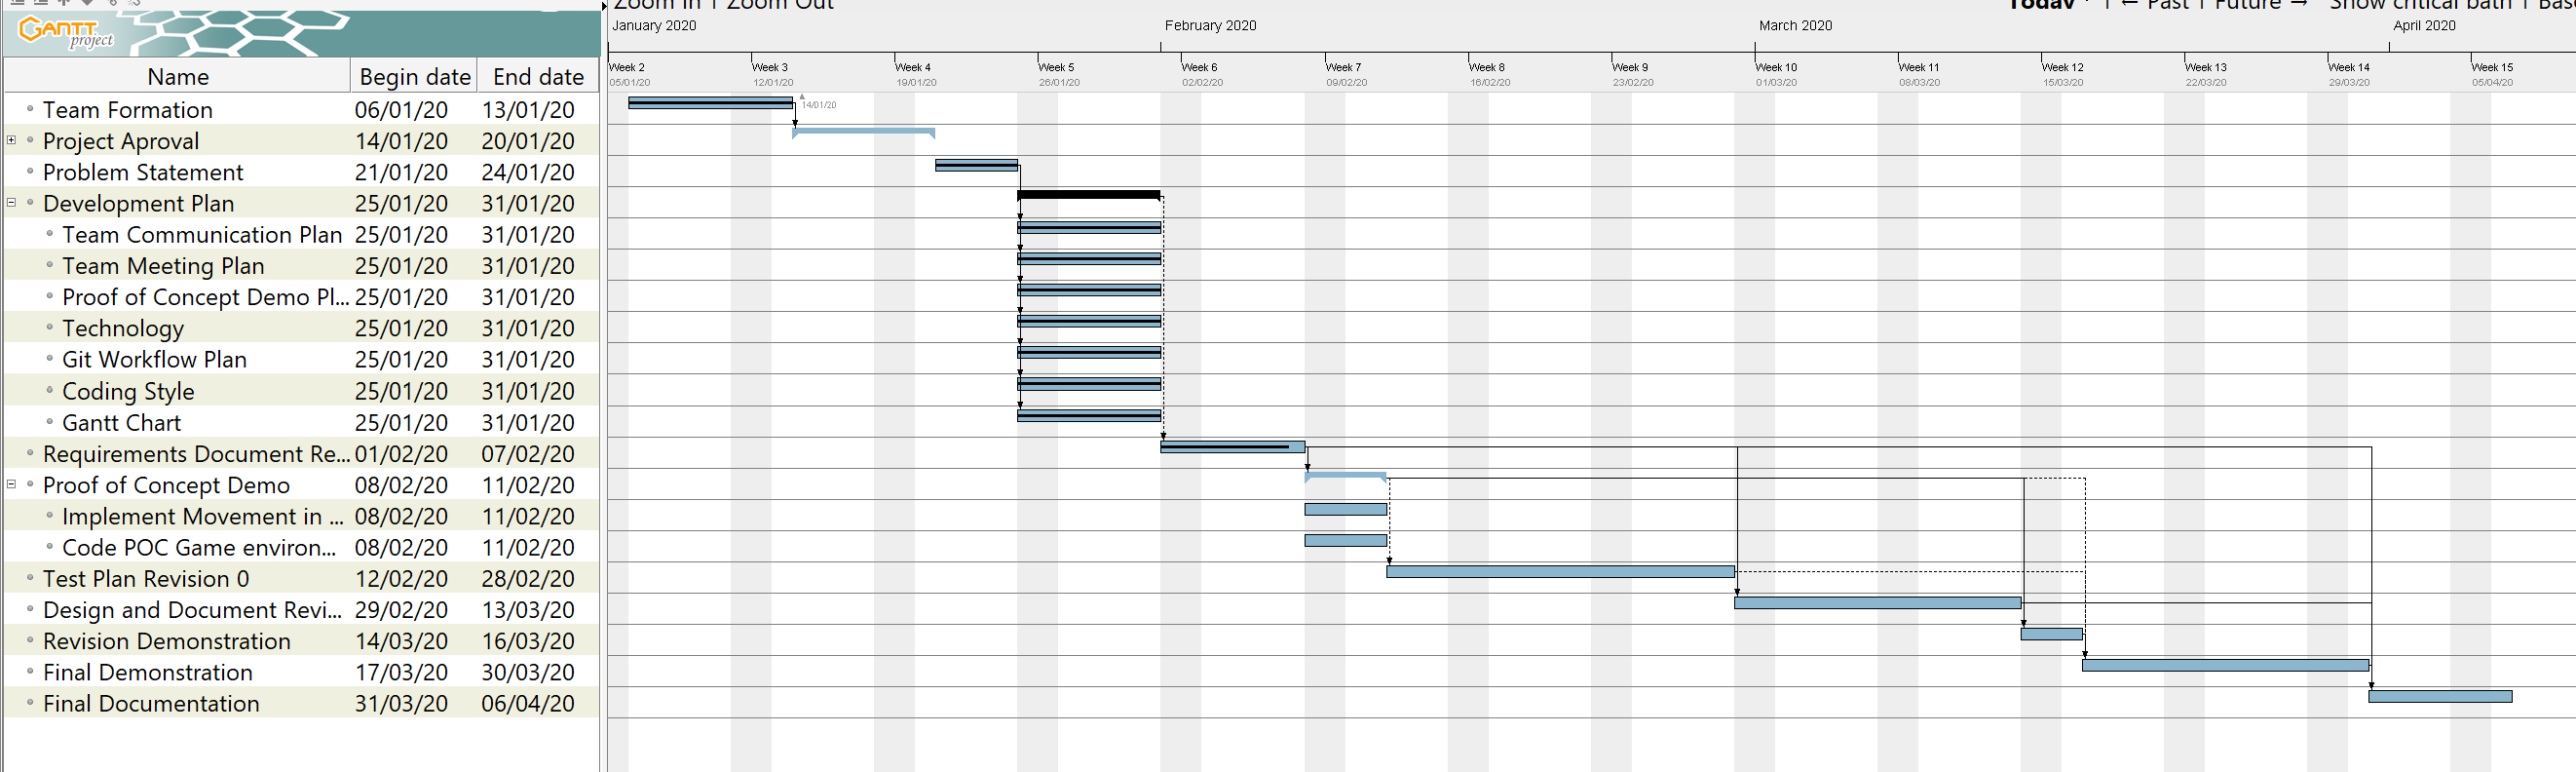
\includegraphics[width=\textwidth]{GanttChartSnapshotFeb9.png}
    \caption{Gantt Chart reflecting Proof of Concept updates}
    \label{fig:ganttchart}
\end{figure}

{\it This Gantt chart is updated throughout the project}

\subsection{Migration to the New Product}
\subsubsection{Requirements for Migration to the New Product}
N/A

\subsubsection{Data That has to Be Modified or Translated for the New System}
N/A

\subsection{Risks}
\subsubsection{Excessive Schedule Pressure}
There are serious time constraints on the project's development period. Therefore, the team be keen to stay on schedule or risk falling behind which would result in the final deliverable not functioning.

Probability: 0 percent

\subsubsection{Low Quality}
If the team looses sight of the end goal and becomes focused on trying to create something in-essential to the project, the main functionality of the end result will be full of issues, such as game lag. This could render the game not playable. Thus, the team must complete the core functions before creating fancy aspects.

Probability: 10 percent

\subsection{Costs}
The entire project will consist of the free to use coding language python and its corresponding free to use library pygame. Therefore, there is no monetary cost to the design and development of the game.

\subsection{User Documentation and Training}
\subsubsection{User Documentation Requirements}
The team will create a game controls outline and add it to the game settings. If the team has time, the first game level might come with a run through tutorial to help first time players understand how to play.

If the game is distributed publicly, a Read-Me file will accompany the game with instructions on how to download and install.

\subsubsection{Training Requirements}
There will be no learning curve; the controls must be intuitive enough to understand without training.

\subsection{Waiting Room}
A story line that plays out as the user beats levels as well as support for mobile devices will not be released as part of this version.

\subsection{Ideas for Solutions}
N/A

\bibliographystyle{plainnat}

\bibliography{SRS}

\newpage

\section{Appendix}

This section has been added to the Volere template.  This is where you can place
additional information.

\subsection{Symbolic Parameters}

The definition of the requirements will likely call for SYMBOLIC\_CONSTANTS.
Their values are defined in this section for easy maintenance.

\end{document}
